\subsubsection{UC12 - Visualizzazione dati del profilo}
\begin{itemize}
\item \textbf{Attori primari}: cliente;
\item \textbf{Descrizione}: il cliente visualizza i suoi dati personali presenti nel sistema;
\item \textbf{Scenario Principale}: il cliente si trova nella pagina del profilo e visualizza i seguenti dati personali:
\begin{itemize}
\item nome;
\item cognome;
\item indirizzo di fatturazione;
\item email.
\end{itemize}
\item \textbf{Precondizione}: il cliente si trova nella pagina del profilo;
\item \textbf{Postcondizione}: vengono visualizzati i dati personali del cliente.
\end{itemize}

\subsubsection{UC13 - Modifica dati del profilo}
\begin{itemize}
\item \textbf{Attori primari}: cliente;
\item \textbf{Descrizione}: il cliente può modificare i dati personali presenti nella sua pagina del profilo;
\item \textbf{Scenario Principale}: il cliente si trova nella pagina del profilo e clicca un tasto dedicato per andare nella pagina di modifica. Da li può modificare le seguenti informazioni:
\begin{itemize}
\item nome [\textbf{UC13.1}];
\item cognome [\textbf{UC13.2}];
\item indirizzo di fatturazione [\textbf{UC13.3}];
\item email [\textbf{UC13.4}];
\item password [\textbf{UC13.5}].
\end{itemize}
Una volta che i campi hanno al suo interno i valori previsti dal cliente, il cliente può premere il pulsante per confermare la modifica dei dati [\textbf{UC13.6}];
\item \textbf{Precondizione}: il cliente si trova nella pagina del profilo;
\item \textbf{Postcondizione}: vengono modificati i dati personali del cliente presenti nel profilo in base alle sue intenzioni.
\end{itemize}

\begin{figure}[H]
\centering
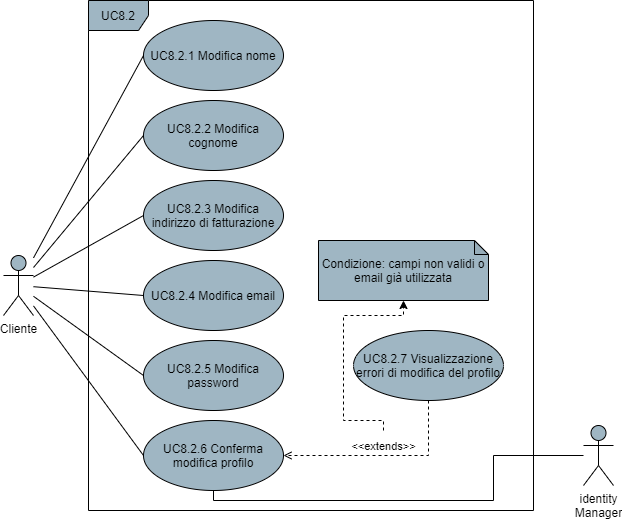
\includegraphics[scale=0.6]{res/UseCase/Immagini/ModificaProfilo}
\caption{Diagramma UML\ped{G} per UC13 - Modifica dati del profilo}
\end{figure}

\subsubsection{UC13.1 - Modifica nome}
\begin{itemize}
\item \textbf{Attori primari}: cliente;
\item \textbf{Descrizione}: il cliente può modificare il nome;
\item \textbf{Scenario Principale}: il cliente visualizza nel campo relativo al nome il dato attualmente presente, che andrà a sovrascrivere con il nuovo nome aggiornato;
\item \textbf{Precondizione}: il cliente si trova nella pagina dedicata alla modifica del profilo;
\item \textbf{Postcondizione}: il cliente ha compilato il campo dedicato al nome, sovrascrivendo il precedente.
\end{itemize}

\subsubsection{UC13.2 - Modifica cognome}
\begin{itemize}
\item \textbf{Attori primari}: cliente;
\item \textbf{Descrizione}: il cliente può modificare il cognome;
\item \textbf{Scenario Principale}: il cliente visualizza nel campo relativo al cognome il dato attualmente presente, che andrà a sovrascrivere con il nuovo cognome aggiornato;
\item \textbf{Precondizione}: il cliente si trova nella pagina dedicata alla modifica del profilo;
\item \textbf{Postcondizione}: il cliente ha compilato il campo dedicato al cognome, sovrascrivendo il precedente.
\end{itemize}

\subsubsection{UC13.3 - Modifica indirizzo di fatturazione}
\begin{itemize}
\item \textbf{Attori primari}: cliente;
\item \textbf{Descrizione}: il cliente può modificare l'indirizzo di fatturazione;
\item \textbf{Scenario Principale}: il cliente visualizza nel campo relativo all'indirizzo di fatturazione il dato attualmente presente, che andrà a sovrascrivere con il nuovo indirizzo aggiornato;
\item \textbf{Precondizione}: il cliente si trova nella pagina dedicata alla modifica del profilo;
\item \textbf{Postcondizione}: il cliente ha compilato il campo dedicato all'indirizzo di fatturazione, sovrascrivendo il precedente.
\end{itemize}

\subsubsection{UC13.4 - Modifica email}
\begin{itemize}
\item \textbf{Attori primari}: cliente;
\item \textbf{Descrizione}: il cliente può modificare l'email;
\item \textbf{Scenario Principale}: il cliente visualizza nel campo relativo all'email il dato attualmente presente, che andrà a sovrascrivere con la nuova email aggiornata;
\item \textbf{Precondizione}: il cliente si trova nella pagina dedicata alla modifica del profilo;
\item \textbf{Postcondizione}: il cliente ha compilato il campo dedicato all'email, sovrascrivendo la precedente.
\end{itemize}

\subsubsection{UC13.5 - Modifica password}
\begin{itemize}
\item \textbf{Attori primari}: cliente;
\item \textbf{Descrizione}: il cliente può modificare la password;
\item \textbf{Scenario Principale}: il cliente visualizza un campo vuoto riguardante la password, che potrà compilare per modificarla;
\item \textbf{Precondizione}: il cliente si trova nella pagina dedicata alla modifica del profilo;
\item \textbf{Postcondizione}: il cliente ha compilato il campo dedicato alla password, sovrascrivendo la precedente.
\end{itemize}

\subsubsection{UC13.6 - Conferma modifica profilo}
\begin{itemize}
\item \textbf{Attori primari}: cliente;
\item \textbf{Descrizione}: il cliente conferma i dati presenti nel form e il profilo viene modificato;
\item \textbf{Scenario Principale}: il cliente preme il pulsante di conferma, la richiesta viene gestita dall'Identity Manager ed il profilo viene modificato con i valori precedentemente inseriti;
\item \textbf{Estensioni}: 
\begin{itemize}
\item se i campi risultano non validi oppure l'email è già stata utilizzata nel sistema, viene mostrato un messaggio di errore [\textbf{UC13.7}].
\end{itemize}
\item \textbf{Precondizione}: il cliente si trova nella pagina dedicata alla modifica del profilo;
\item \textbf{Postcondizione}: il cliente ha modificato il profilo con i dati inseriti.
\end{itemize}

\subsubsection{UC13.7 - Visualizzazione errori di modifica del profilo}
\begin{itemize}
\item \textbf{Attori primari}: cliente;
\item \textbf{Descrizione}: il cliente visualizza un errore riguardante i campi di modifica profilo che ha inserito. Questi errori possono essere:
\begin{itemize}
\item \textbf{Campo non valido}: un campo risulta vuoto o con caratteri non validi;
\item \textbf{Email già utilizzata}: l'email è già stata utilizzata da un altro cliente.
\end{itemize}
\item \textbf{Scenario Principale}: il sistema riconosce uno o più errori nei campi inseriti dal cliente e vengono visualizzati nella pagina di modifica profilo;
\item \textbf{Precondizione}: il cliente ha inserito i campi ed ha provato ad effettuare la modifica del profilo;
\item \textbf{Postcondizione}: viene visualizzato un messaggio di errore nella pagina di modifica del profilo e i dati non sono stati modificati.
\end{itemize}

\subsubsection{UC14 - Visualizzazione ordini effettuati dall'utente}
\begin{itemize}
\item \textbf{Attori primari}: cliente;
\item \textbf{Descrizione}: il cliente può visualizzare una lista di ordini effettuati;
\item \textbf{Scenario Principale}: il cliente si trova nella pagina del profilo e visualizza una lista di ordini effettuati. Per ogni ordine vengono visualizzati una serie di dati [\textbf{UC14.1}];
\item \textbf{Precondizione}: il cliente si trova nella pagina del profilo e ha effettuato almeno un ordine nel sito;
\item \textbf{Postcondizione}: viene visualizzata una lista di tutti gli ordini che il cliente ha effettuato.
\end{itemize}

\begin{figure}[H]
\centering
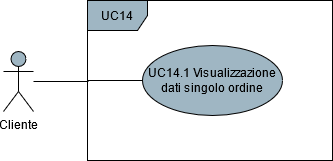
\includegraphics[scale=0.6]{res/UseCase/Immagini/VisualizzazioneOrdini}
\caption{Diagramma UML\ped{G} per UC14 - Visualizzazione ordini effettuati dall'utente}
\end{figure}

\subsubsection{UC14.1 - Visualizzazione dati singolo ordine}
\begin{itemize}
\item \textbf{Attori primari}: cliente;
\item \textbf{Descrizione}: per ogni ordine nella lista degli ordini effettuati, vengono visualizzati una serie di dati;
\item \textbf{Scenario Principale}: Il cliente si trova nella pagina del profilo e, cliccando un ordine effettuato, visualizza  una pagina di riepilogo con i seguenti dati:
\begin{itemize}
\item id ordine;
\item prodotti acquistati;
\item quantità prodotti acquistati;
\item costo per prodotto;
\item costo totale;
\item tasse applicate;
\item data d'acquisto.
\end{itemize}
\item \textbf{Precondizione}: il cliente, cliccando su un ordine nella sua pagina di profilo, si trova nella pagina di riepilogo di un ordine;
\item \textbf{Postcondizione}: vengono visualizzati i dati dell'ordine scelto.
\end{itemize}

\subsubsection{UC15 - Eliminazione account}
\begin{itemize}
\item \textbf{Attori primari}: cliente;
\item \textbf{Descrizione}: il cliente può eliminare il suo account dal sistema;
\item \textbf{Scenario Principale}: il cliente si trova nella pagina del profilo e clicca il tasto dedicato per mandare la richiesta di eliminazione dell'account all'Identity Manager;
\item \textbf{Precondizione}: il cliente si trova nella pagina del profilo;
\item \textbf{Postcondizione}: l'account è stato eliminato dal sistema e il cliente diventa un utente non autenticato.
\end{itemize}
